\newcommand{\winw}[2]{\textsf{window}_{#1}{(#2)}}
\newcommand{\win}[1]{\textsf{window}{(#1)}}
\newcommand{\str}[1]{\textsf{string}{(#1)}}
\newcommand{\prem}[1]{\textsf{prem}~#1}
\newcommand{\conc}[1]{\textsf{conc}~#1}
\newcommand{\rewHead}[3]{\textsf{rewHead}~#1~(#2)~(#3)}
\newcommand{\rewAt}[4]{\textsf{rewAt}~#1~#2~#3~#4}
\newcommand{\prefix}[2]{\textsf{prefix}~#1~#2}

\newcommand{\strentE}[1]{\rightsquigarrow_{#1}^E}
\renewcommand{\strent}[1]{\rightsquigarrow_{#1}}

\newcommand{\pFlip}[1]{\textsf{pFlip}~#1}
\newcommand{\pFlipi}[1]{\text{\textasciitilde}#1}
\newcommand{\pRev}{\textsf{pRev}}

\newcommand{\nilstr}[2]{E~#1~#2}

\newcommand{\divides}{\mid}
\newcommand{\notdivides}{\nmid}

\newcommand{\Rtape}{\ensuremath{R_{\text{t}}}}

\newcommand{\trewwin}[6]{
  \begin{tikzpicture}
    \draw[thick] (0, 0) -- (2.25, 0);
    \draw (0.75, -0.75) -- (0.75, 0.75);
    \draw (1.5, -0.75) -- (1.5, 0.75);
    \node at (0.375, 0.375) {\ensuremath{#1}};
    \node at (0.375, -0.375) {\ensuremath{#4}};
    \node at (1.125, 0.375) {\ensuremath{#2}};
    \node at (1.125, -0.375) {\ensuremath{#5}};
    \node at (1.875, 0.375) {\ensuremath{#3}};
    \node at (1.875, -0.375) {\ensuremath{#6}};
  \end{tikzpicture}
}

\newcommand*{\irewwin}[6]{\ensuremath{[#1, #2, #3]~/~[#4, #5, #6]}}
\chapter{Reducing GenNP to Parallel Rewriting}\label{chap:gennp_pr}
We introduce the string-based \emph{Parallel Rewriting} (\PR{}) problem which formally captures the idea of a string tableau constrained by rewrite windows. The rest of this chapter is then devoted to formalising the tableau construction presented in Chapter~\ref{chap:informaloverview} and proving its correctness in a reduction from \gennp{} to \PR{}.

\section{Parallel Rewriting}\label{sec:pr}
Parallel Rewriting works over a finite alphabet $\Gamma$. Given an initial string $x_0$, a set of rewrite windows $R$, a number of steps $t$, and a final constraint $\Rfinal$, we are tasked with determining whether there exists a sequence of valid rewrites $x_0 \strent{} \ldots \strent{} x_t$ such that $x_t$ satisfies a substring constraint $\Rfinal$, written $x_t \models \Rfinal$.

\begin{definition}[Parallel Rewriting instances]\label{def:pr}
  $p = (\Sigma, o, w, x_0, R, \Rfinal, t)$ is a Parallel Rewriting instance, where 
  \begin{itemize}
    \item $\Sigma : \textsf{finType}$ is the finite alphabet,
    \item $o : \nat$ with $o > 0$ is the rewriting offset,
    \item $\omega : \nat$ with $\omega > 0$ is the width of rewriting windows,
    \item $x_0 : \str{\Sigma}$ with $\length{x_0} \ge \omega$ is the initial string, 
    \item $R : \listsof{\winw{\omega}{\Sigma}}$ is the set of rewrite windows,
    \item $\Rfinal : \listsof{\str{\Sigma}}$ is a set of final substrings,
    \item $t : \nat$ is the number of rewrite steps, 
  \end{itemize}
  if $o \divides w$ and $o \divides \length{x_0}$. 
Here, $\winw{\omega}{\Sigma} := {\Sigma}^\omega \times {\Sigma}^\omega$ denotes the type of windows of width $w$ over $\Sigma$ and $\str{\Sigma} := \listsof{\Sigma}$. 
\end{definition}
If it is clear from the context, we write $\win{\Sigma}$ instead of $\winw{\omega}{\Sigma}$, omitting the width.
Instead of directly using the projections $\pi_1$ and $\pi_2$ on a window $w$, we usually write $\prem{w}$ and $\conc{w}$. 

Abstractly, $o$ symbols are always grouped together to form one abstract symbol, explaining the divisibility constraints. Throughout this chapter, we always work with a offset of 1 and the more general case will only become relevant in Chapter~\ref{chap:pr_bpr}.

Let us fix the structural parameters $\Sigma$, $o$ and $\omega$ satisfying the conditions stated in the definition for the rest of the section.

\subsection{Validity}

\begin{definition}[Matching Windows]
  \begin{gather*}
    \rewHead{w}{a}{b} \defeq \prefix{(\prem{w})}{a} \land \prefix{(\conc{w})}{b} \\
    \prefix{s}{t} \defeq \exists b, t = s \concat{} b,
  \end{gather*}
  that is, a window $w$ justifies a rewrite at the head of two strings $a$ and $b$ if it matches the heads of $a$ and $b$.

  A windows $w$ justifies a rewrite at position $i$ of strings $a, b$ if it matches the head of the strings starting from position $i$:
    $\rewAt{w}{i}{a}{b} \defeq \rewHead{w}{a[i..]}{b[i..]}$
\end{definition}
\todo{maybe mention the facts (tail invariance, ...) which are routinely used?}

\begin{definition}[Validity (Explicit Characterisation)]
  Given a set of rewrite windows $R$, the validity of a rewrite of $a : \str{\Sigma}$ to $b : \str{\Sigma}$, written $a \strentE{R} b$, is defined by:
  \begin{align*}
    a \strentE{R} b \defeq \quad& \length{a} = \length{b} \\
    \land \quad & (\exists k, \length{a} = k \cdot o) \\
    \land \quad & \forall 0 \le i = j \cdot o < \length{a} + 1 - \omega, \exists w, w \in R \land \rewAt{w}{i}{a}{b} 
  \end{align*}
  \todo{$\le \length{a} - \omega$ would be more readable, but is wrong when using truncating subtraction. Which convention should be used?}
\end{definition}

Intuitively, the definition says that a rewrite is possible if we can find a rewrite window justifying a local rewrite for every possible offset. ``Possible offsets'' are those in the range $[0, \length{a} - \omega]$, as the windows have a width of $\omega$. Additionally, the rewrites need only be possible at multiples of the offset, again supporting the view that $o$ symbols together form a unit.

Note that the dependency on $o$ and $\omega$ is not made explicit in the notation, instead they need to be inferred from the context. If the set of rewrite windows $R$ is clear, we may also drop that.

While this definition is fairly intuitive, it does not support easy inductive reasoning. Therefore, we use an equivalent inductive definition.

\begin{definition}[Validity] 
  Given a set of rewrite windows $R$, the validity of a rewrite of $a : \str{\Sigma}$ to $b : \str{\Sigma}$, written $a \strent{} b$, is defined inductively:  
  \begin{gather*}
    \infer{\nil \strent{R} \nil}{} \\
    \infer{u\concat{} a \strent{R} v \concat{} b}{a \strent{R} b \quad \length{a} < \omega - o \quad \length{u} = o \quad \length{v} = o} \\
    \infer{u \concat{} a \strent{R} v \concat{} b}{a \strent{R} b \quad \length{u} = o \quad \length{v} = o \quad w \in R \quad \rewHead{w}{u\concat{}a}{v \concat{} b}}.
  \end{gather*}
\end{definition}

This version prepends a chunk of $o$ symbols in each step. The first two cases deal with proving validity of rewrites in strings of length $< \omega$. The third case is the interesting one and is defined in the intuitive way.

\begin{remark}
  It might seem peculiar that we do not require the strings to have a minimum length of $\omega$: strings of length $< \omega$ can be rewritten vacuously to any other string as they are covered by no window. 
  This enables us to only mention $\textsf{rewHead}$ in the successor case of the inductive definition; otherwise, we would also need it in the base case. This simplifies the main proofs throughout this chapter considerably, albeit at the cost of having nonsensical base cases.
\end{remark}

\begin{proposition}[Vacuous Rewriting]\label{lem:vacuous}
  Let $a, b : \str{\Sigma}$ with $\length{a} = \length{b} = k \cdot o < \omega$. Then $a \strent{} b$. 
\end{proposition}
\begin{proof}
  By induction on $m$.
\end{proof}

\begin{proposition}[Length Invariance]
  Let $a, b : \str{\Sigma}$ with $a \strent{} b$. Then $\length{a} = \length{b}$. 
\end{proposition}

\begin{lemma}[Agreement of $\strentE{}$ and $\strent{}$]\label{lem:agree_valid}
  For any set of rewrite windows $R$, it holds that 
  \[a \strentE{R} b \leftrightarrow a \strent{R} b. \]
\end{lemma}
\begin{proof}
  \begin{description}
    \item[$\rightarrow$:]
      By definition, we have $k$ with $\length{a} = k \cdot o$. The proof is by induction on $k$ with $a$ and $b$ quantified.
    \item[$\leftarrow$:]
      By induction on $a \strentE{R} b$. 
  \end{description}
\end{proof}


\subsection{Parallel Rewriting}
\todo{subsection is named the same as section}
Parallel Rewriting generates a sequence of strings. The last string should contain one element of a set of strings as a substring.
\begin{definition}[Substring constraint]
  Given a set of strings $\Rfinal : \listsof{\str{\Sigma}}$, string $s$ satisfies $\Rfinal$, written $s \models \Rfinal$, if:
  \[\exists \mathit{subs}~k, \mathit{subs} \in \Rfinal \land k \cdot o \le \length{s} \land \prefix{\mathit{subs}}{s[k \cdot o..]} \]
\end{definition}
The definition requires a string to be a substring at a position which is a multiple of the offset $o$.

\begin{definition}[Parallel Rewriting]
  \[\PR{}~(\Sigma, o, \omega, x_0, R, \Rfinal, t) \defeq \exists x_t, x_0 \strent{R}^t x_t \land x_t \models \Rfinal, \]
  where we implicitly require the instance to satisfy the syntactic constraints of Definition~\ref{def:pr}. 
  \todo{should that be a more explicit part as in the coq development?}
\end{definition}

One can interpret \PR{} to be a problem between Turing machines and circuits: of course, the definition over a finite alphabet still closely resembles Turing machines. However, in contrast to Turing machines, Parallel Rewriting can completely rewrite the string in a single step, although the power of this is limited as it operates on strings of a fixed size. 
Circuits, on the other hand, are similar in the sense that they also work in parallel. The fact that adjacent rewrite positions overlap and can thus enforce a global constraint in a single rewrite step is unlike circuits, though. 

\subsection{3-\PR{}}
For the rest of this chapter, we fix the width to $3$ and the offset to $1$, which are the parameters needed for the Turing machine encoding. We call this variant 3-\PR{}. 
The inductive definition of validity can be simplified a bit:
\begin{align*}
  \infer{\nil \strent{R} \nil}{} \quad
  \infer{x::a \strent{R} y ::b}{a \strent{R} b \quad \length{a} < 2} \quad
  \infer{x::a \strent{R} y :: b}{a \strent{R} b \quad w \in R \quad \rewHead{w}{x::a}{y::b}}
\end{align*}

We use the notation introduced in the previous chapter to denote the window $((x_1, x_2, x_3), (x_4, x_5, x_6))$: 
\begin{center}
  \trewwin{x_1}{x_2}{x_3}{x_4}{x_5}{x_6}
\end{center}
Sometimes, we also use $\irewwin{x_1}{x_2}{x_3}{x_4}{x_5}{x_6}$ if we need to write down a window in-line.

\section{Encoding Tapes and Configurations}
We move to the construction of the Turing machine simulation. Our goal is to devise and verify a 3-\PR{} instance simulating a Turing machine. 
For the rest of the chapter, let us fix a \gennp{} instance consisting of a finite tape alphabet $\Sigma$, a single-tape Turing machine $M = (Q, \delta, q_0, \textsf{halt})$ over $\Sigma$, a number $t$ of steps, and a maximum size $k$ of the input. 

Formalising the intuitions from Chapter~\ref{chap:informaloverview}, we define the alphabet $\Gamma$ of the Parallel Rewriting instance for the deterministic simulation\footnote{This does not include the part for generating the initial configuration.}.

\newcommand{\stateSigma}{\Sigma_{\mathit{state}}}
\newcommand{\delimSigma}{\Sigma_{\mathit{delim}}}
\newcommand{\tapeSigma}{\Sigma_{\mathit{tape}}}
\newcommand{\States}{\textsf{States}}

\begin{align*}
  \polarity &\defeq + \bnfmid - \bnfmid \circ \\
  \textsf{delim} &\defeq \# \\
  \stateSigma &\defeq \opt{\Sigma} \\
  \States &\defeq Q \times \stateSigma \\
  \tapeSigma &\defeq \polarity \times \stateSigma \\
  \delimSigma &\defeq \textsf{delim} + \tapeSigma \\
  \Gamma &\defeq \States + \delimSigma
\end{align*}

We need the subalphabets at various points. When we write down elements of $\Gamma$, we leave the injections into the sum types and option types implicit. Sometimes, we also implicitly lift functions from a smaller alphabet to a larger one.
We use the metavariables $\sigma : \Sigma$, $m : \tapeSigma$, $p : \polarity$, $\gamma : \Gamma$, $u : \str{\Sigma}$, and $h : \str{\Gamma}$. 
Given $m$, we write $\polpos{m}$ for $(+, m)$, $\polneg{m}$ for $(-, m)$, and $\polneut{m}$ for $(\circ, m)$. 

\begin{definition}[Polarity Reversion]
  \begin{align*}
    \pFlip{p} &\defeq \match p \withl \circ~\Rightarrow \circ \withm +~\Rightarrow - \withm -~\Rightarrow +\withr \\
    \pRev~h &\defeq \rev{\withl\pFlip{x} \bnfmid x \in h\withr}
  \end{align*}
  Notationally, we write $\pFlipi{p}$ for $\pFlip{p}$. 
\end{definition}
$\pRev$ reverses a string and flips the polarities the symbols are annotated with: $\pRev~[\polpos{m_1}, \polpos{m_2}] = [\polneg{m_2}, \polneg{m_1}]$. 
Note that we are already using an implicit lifting of $\pFlip{}$ in the definition of $\pRev$. 

\begin{fact}[Involutions]\label{fact:prev_involution}
  $\pFlip{}$ and $\pRev{}$ are involutions, that is, $\pFlip{(\pFlip{p})} = p$ and $\pRev{(\pRev~h)} = h$. 
\end{fact}

Figure~\ref{fig:configlayout} shows the layout of a configuration string again. We refer to the center symbol as the \emph{state symbol} and to the substrings left and right of it as the \emph{left tape half} and the \emph{right tape half}.
In dependence of $t$ and $k$, we define the following numbers:
\begin{align*}
  z &\defeq t + k \\
  \forall n, \hat{n} &\defeq n + 2 \\
  l &\defeq 2 \cdot (\hat{z} + 1) + 1
\end{align*}
$z$ is the amount of space available for the Turing machine and thus $z$ units of space need to be available to the left and to the right in the configuration string as the tape can be shifted to be completely on one side of the state symbol.
For technical reasons, we want three symbols to be available to either side of the state symbol even if $t = k = 0$. One of those symbols will be the delimiter $\#$, the other two are additional blanks which will never be used by the Turing machine. Thus $\hat{z}$ is the number of symbols on each side excluding the delimiter. 
Finally, $l$ is the length of the whole configuration string including the center state symbol.

\begin{figure}
  \begin{center}
    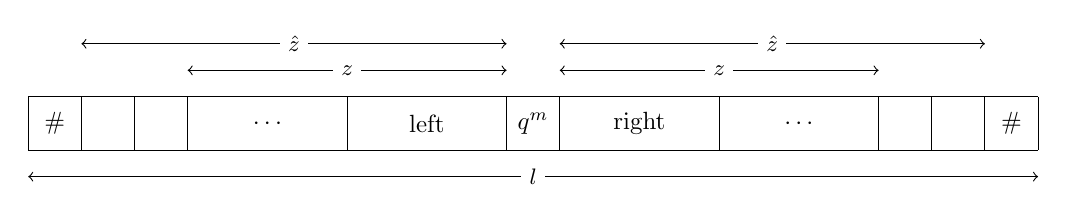
\begin{tikzpicture}[scale=0.9, every node/.style={scale=0.9}]
      \draw (-1.5, 0) -- (12.75, 0);
      \draw (-1.5, 0) -- (-1.5, 0.75);
      \draw (-1.5, 0.75) -- (12.75, 0.75);
      \draw (12.75, 0.75) -- (12.75, 0);

      \draw (0.75, 0) -- (0.75, 0.75);
      \draw (10.5, 0) -- (10.5, 0.75);
      \draw (0, 0) -- (0, 0.75);
      \draw (11.25, 0) -- (11.25, 0.75);
      \draw (-0.75, 0) -- (-0.75, 0.75);
      \draw (12, 0) -- (12, 0.75);

      \draw (6, 0) -- (6, 0.75);
      \draw (5.25, 0) -- (5.25, 0.75);

      \draw (3, 0) -- (3, 0.75);
      \draw (8.25, 0) -- (8.25, 0.75);

      \node at (-1.125, 0.375) {\#};
      \node at (-0.375, 0.375) {\blank};
      \node at (0.375, 0.375) {\blank};
      \node at (5.625, 0.375) {$q^m$};
      \node at (12.375, 0.375) {\#};
      \node at (11.625, 0.375) {\blank};
      \node at (10.875, 0.375) {\blank};

      \node at (1.125, 0.375) {\blank};
      \node at (1.875, 0.375) {$\cdots$};
      \node at (2.625, 0.375) {\blank};

      \node at (8.625, 0.375) {\blank};
      \node at (9.375, 0.375) {$\cdots$};
      \node at (10.125, 0.375) {\blank};

      \node at (4.125, 0.375) {left};
      \node at (7.125, 0.375) {right};
      
      \path[<->] (-0.75, 1.5) edge node[fill=white, anchor=center, pos= 0.5] {\small $\hat{z}$} (5.25, 1.5);
      \path[<->] (0.75, 1.125) edge node[fill=white, anchor=center, pos=0.5] {\small $z$} (5.25, 1.125);
      \path[<->] (6, 1.5) edge node[fill=white, anchor=center, pos= 0.5] {\small $\hat{z}$} (12, 1.5);
      \path[<->] (6, 1.125) edge node[fill=white, anchor=center, pos=0.5] {\small $z$} (10.5, 1.125);
      \path[<->] (-1.5, -0.375) edge node[fill=white,anchor=center, pos=0.5] {\small $l$} (12.75, -0.375);


    \end{tikzpicture}
  \end{center}
  \caption{Layout of a configuration string.}\label{fig:configlayout}
\end{figure}

In order to make reasoning about configuration strings possible, we define representation relations for tape halves and configurations.

\begin{definition}[Tape Representation]
  \begin{align*}
    u \reprtt{w}{p} h &\defeq \length{u} \le w \land h = \withl(p, x) \withm x \in u\withr \concat \nilstr{p}{(\hat{w} - \length{u})}\\
  u \reprt{p} h &\defeq u \reprtt{z}{p}, 
  \end{align*}
  where $E$ is the string representing the empty tape:
  \begin{align*}
    \nilstr{p}{0} &\defeq [\#] \\
    \nilstr{p}{(\natS{n})} &\defeq (p, \blank) :: \nilstr{p}{n}
  \end{align*}
\end{definition}
$u \reprtt{w}{p} h$ means that $h$ contains the elements of $u$ annotated with polarity $p$ where a total of $w$ symbols are available for the simulation to use.
For the correctness statements, we use $u \reprt{p} h$, but usually generalise to $u \reprtt{w}{p} h$ for some $w$ in inductive proofs. 

\begin{proposition}\label{prop:tapefacts}\leavevmode
  \begin{itemize}
    \item $\withl \pFlip{\gamma} \withm \gamma \in \nilstr{p}{n} \withr = \nilstr{(\pFlip~p)}{n}$
    \item $u \reprtt{w}{p} h \rightarrow \length{h} = \natS{\hat{w}}$
    \item $u \reprtt{w}{p} h \rightarrow u \reprtt{w}{\pFlip{p}} \withl \pFlip{\gamma} \withm \gamma \in h \withr$
  \end{itemize}
\end{proposition}
\todo{maybe unique representation of the empty tape}

\begin{definition}[Configuration Representation]
  \begin{align*}
    (q, tp) \reprc{} (l, e, r) &\defeq \exists p, e = (q, \tmcurrent{tp}) \land \tmleft{tp} \reprt{p} l \land \tmright{tp} \reprt{p} r \\
    c \reprc{} s &\defeq \exists l~ e~ r, s = \rev~{l} \concat{} [e] \concat{} r \land (q, tp) \reprc{} (l, e, r) 
  \end{align*}
\end{definition}
A configuration $c = (q, tp)$ is represented by a string containing the state symbol in the center with strings representing the left and right tape halves left and right of it. Note that the left tape half is reversed: while the Turing machine tapes have the symbol closest to the machine head at the head of the list, we need the symbol closest to the head to be next to the string's center. This will pose some difficulties later on.

\section{Modifying Tapes}
In this section, we introduce the rewrite rules for shifting tape halves and prove the main results for adding symbols to the representation of a tape half.

\subsection{Tape Rules}
The rules are annotated with the tape halves they can be used on. These annotations have no formal meaning but help with the intuition.

\paragraph{Right Shifts}
\begin{center}
\begin{tabular}{cc}
\trewwin{\sigma_1}{\sigma_2}{\sigma_3}{\polpos{\sigma_4}}{\polpos{\sigma_1}}{\polpos{\sigma_2}} 
  \quad \trewwin{\blank}{\blank}{\blank}{\polpos{\blank}}{\polpos{\blank}}{\polpos{\blank}}
  & (both halves) \\
\trewwin{\blank}{\blank}{\blank}{\polpos{\sigma_1}}{\polpos{\blank}}{\polpos{\blank}} 
  \quad \trewwin{\sigma_1}{\blank}{\blank}{\polpos{\sigma_2}}{\polpos{\sigma_1}} {\polpos{\blank}}
\quad \trewwin{\sigma_1}{\sigma_2}{\blank}{\polpos{\sigma_3}}{\polpos{\sigma_1}}{ \polpos{\sigma_2}}
  & (right half) \\
\trewwin{\blank}{\blank}{\sigma_1}{\polpos{\blank}}{\polpos{\blank}}{\polpos{\blank}}
  \quad \trewwin{\blank}{\sigma_1}{\sigma_2} {\polpos{\blank}}{\polpos{\blank}}{ \polpos{\sigma_1}} 
\quad \trewwin{\sigma_1}{\sigma_2}{\sigma_3}{\polpos{\blank}}{\polpos{\sigma_1}}{ \polpos{\sigma_2}}
  & (left half)
\end{tabular}
\end{center}
\todo{fix formatting}

The rules implicitly encode the invariant that all symbols used by the Turing machine are placed contiguously with no blanks inbetween. For instance, we do not need the following two rules:
\begin{center}
  \trewwin{\sigma_1}{\blank}{\sigma_2}{\polpos{\blank}}{\polpos{\sigma_1}}{\polpos{\blank}}
  \quad
  \trewwin{\sigma_1}{\blank}{\blank}{\polpos{\blank}}{\polpos{\sigma_1}}{\polpos{\blank}}
\end{center}
In the first case, the premise prevents the rule from ever being applicable. In the second case, the overlap of the rewrite windows and the state symbol which stands between both tape halves is the reason. 
We call such instantiations of a rewrite rule \emph{spurious}.

Knowing this, we write down the above rules in a more succinct way as 
\begin{center}
  \trewwin{m_1}{m_2}{m_3}{\polpos{m_4}}{\polpos{m_1}}{\polpos{m_2}}
\end{center}
While we would be fine having the spurious rewrite windows, they do make additional reasoning necessary in some cases. Therefore, we just regard this as a notation for the expanded form above, instead of actually seeing spurious instantitions as valid. One can easily derive the rules which are actually relevant.

\paragraph{Left Shifts}
We only write down the abbreviated form:
\begin{center}
  \trewwin{m_1}{m_2}{m_3}{\polneg{m_2}}{\polneg{m_3}}{\polneg{m_4}}
\end{center}
Note that this rule exactly mirrors the rule for shifting the tape to the right.
\paragraph{Identity Rules}
\begin{center}
  \trewwin{m_1}{m_2}{m_3}{\polneut{m_1}}{\polneut{m_2}}{\polneut{m_3}}\\
  \trewwin{\#}{\blank}{\blank}{\#}{\blank}{\blank} 
  \quad \trewwin{\blank}{\blank}{\#}{\blank}{\blank}{\#}
\end{center}
We need no windows which contain both the delimiter $\#$ and an element of $\Sigma$ as the Turing machine by construction cannot use the two blanks adjacent to the delimiters.

The collection of all windows generated by these rules is referred to as $\Rtape$. 
Throughout the rest of this section, we implicitly always use $\Rtape$ as the set of rewrite windows when talking about validity.

\begin{remark}
  It now becomes clear why we need the delimiter $\#$. Without it, symbols could just be introduced at the edge of the string. For instance, the rule 
  \begin{center}
    \tikzset{baseline={([yshift=-22pt]current bounding box.north)}}
    \trewwin{\blank}{\blank}{\blank}{\polpos{\sigma_1}}{\polpos{\blank}}{\polpos{\blank}},
  \end{center}
  which is intended for use on the right tape half, could then also be used at the leftmost position of the left tape half as no rewrite window is overlapping from the left.
\end{remark}

\begin{lemma}[Symmetry of \Rtape]\label{lem:symm_rtape}
  \[\irewwin{\gamma_1}{\gamma_2}{\gamma_3}{\gamma_4}{\gamma_5}{\gamma_6} \in \Rtape \leftrightarrow \irewwin{\pFlipi{\gamma_3}}{\pFlipi{\gamma_2}}{\pFlipi{\gamma_1}}{\pFlipi{\gamma_6}}{\pFlipi{\gamma_5}}{\pFlipi{\gamma_4}} \in \Rtape \]
\end{lemma}
\begin{proof}
  We first prove one direction and then use that $\pFlip$ is involutive.
  By inversion on the rule used to generate the window. The interesting case is the one for shifting the tape to the left or to the right, which follows by the fact that the rules for shifting to the left and shifting to the right are exactly symmetric. 
\end{proof}

%lemma 15 from memo
\begin{lemma}[Symmetry of Tape Rewrites]\label{lem:symm_tape_rew}\leavevmode
  \begin{enumerate}[1)]
    \item $h \strent{\Rtape} h' \rightarrow \pRev~h \strent{\Rtape} \pRev~h'$ 
    \item $\pRev~h \strent{\Rtape} \pRev~h' \rightarrow h \strent{\Rtape} h'$
    \item $h \strent{\Rtape} h' \rightarrow \withl \pFlip{x} \withm x \in h \withr \strent{\Rtape} h'$
  \end{enumerate}
\end{lemma}
\begin{proof}
  \begin{enumerate}[1)]
    \item By induction on $h \strent{\Rtape} h'$. The first two cases are trivial. 
      In the successor case, there is the problem that the new symbols are appended at the end of the strings, while the inductive definition of $\strent{}$ only allows to prepend new symbols. We switch to the explicit characterisation by Lemma~\ref{lem:agree_valid} and do a case analysis on the position for which we need to provide a rewrite window. For all but the last position, we can apply the inductive hypothesis, while we use the polarity-reversed new rewrite window, which exists by Lemma~\ref{lem:symm_rtape}, for the last position.
    \item Apply 1) and use that $\pRev$ is an involution.
    \item By induction on $h \strent{\Rtape} h'$ and inversion on the used rewrite rule.
  \end{enumerate}
\end{proof}

If we want to prove a statement for the left and the right tape half, Lemma~\ref{lem:symm_tape_rew} allows us to just derive the statement for the right tape half and then get the symmetric result for the left tape half for free. This is helpful in particular because we cannot do direct inductions over the reversed left tape halfs. 

\subsection{Manipulation of Tape Representations}

We prove several lemmas which are similar in flavour and will later be the base cases of more general results. They state that, starting from a blank tape half, we can leave the tape half unchanged, add a symbol of $\Sigma$, or remove a symbol. Moreover, if a blank tape half rewrites to a string of which the first symbol is known, the rest of the string is also uniquely determined. This is just an instance of the more general observation that the rewrite rules introduced up to now only allow for deterministic rewrites.
These results are each proven for the right tape half and then derived for the left tape half by Lemma~\ref{lem:symm_tape_rew}. 

\begin{remark}
  It now becomes clear why we require at least three symbols on each side of the state symbol: this way, we can prove results about each of the tape halves individually without running into the problem of vacuous rewrites~(Lemma~\ref{lem:vacuous}). 
\end{remark}

%lemma 16
\begin{lemma}[Empty Tape Half: Blank Rewriting]\label{lem:nilstr_blank}\leavevmode
  \begin{enumerate}
    \item $\nilstr{p}{\hat{n}} \strent{\Rtape} \nilstr{p'}{\hat{n}}$ and $\nilstr{p}{\hat{n}} \strent{\Rtape} (p', \blank) :: s \rightarrow s = \nilstr{p'}{(\natS{n})}$
    \item $\rev~{(\nilstr{p}{\hat{n}})} \strent{\Rtape} \rev~{(\nilstr{p}{\hat{n}})}$ and $\rev~{(\nilstr{p}{\hat{n}})} \strent{\Rtape} \rev~{((p', \blank) :: s)} \rightarrow s = \nilstr{p'}{(\natS{n})}$
  \end{enumerate}
\end{lemma}
\begin{proof}
  \begin{enumerate}
    \item The first statement follows by induction on $n$. For the second one, we unfold $\hat{n} = \natS{(\natS{n})}$ and generalise $\natS{n}$ to arbitrary $n \ge 1$. The statement then follows by induction on $n$: the base case is contradictory. In the successor case, we do another case analysis on $n$. If $n =0$, the statement follows by inversion on the used rewrite rule. 
      Otherwise, $n = S n'$. We have $\nilstr{p}{(3+n')} \strent{} (p', \blank) :: s$ and show $s = \nilstr{p'}{(2 + n)}$. By inversion on the rewrite rule used at the head, we get four cases and in each one, $s = (p', \blank) :: s'$ and $\nilstr{p}{(2+n)} \strent{} (p', \blank) :: s'$. As $S n' \ge 1$, we apply the inductive hypothesis and get $s' = \nilstr{p'}{(\natS{n})}$, closing the proof. 
    \item For the first statement, it suffices to show $\rev~{(\nilstr{(\pFlipi{\pFlipi{p}})}{\hat{n}})} \strent{\Rtape} \rev~{(\nilstr{(\pFlipi{\pFlipi{p}})}{\hat{n}})}$. By Proposition~\ref{prop:tapefacts}.1), we can pull out one of the $\pFlip$s to turn the $\rev$ into a $\pRev$. Applying Lemma~\ref{lem:symm_tape_rew}.1), we are left with $\withl \pFlipi{\gamma} \withm \gamma \in \nilstr{p}{\hat{n}} \withr \strent{\Rtape} \withl \pFlipi{\gamma} \withm \gamma \in \nilstr{p'}{\hat{n}} \withr$. This follows by another application of Proposition~\ref{prop:tapefacts}.1) and part 1). 

      The second part is proved in a similar way: we use that $\pFlip$ is involutive, apply Lemma~\ref{lem:symm_tape_rew}.2), and use part 1).
  \end{enumerate}
\end{proof}

The important idea of Lemma~\ref{lem:nilstr_blank} is that the rewrite is uniquely determined \emph{once we know the first symbol} of the target string. All of the important lemmas in the remainder of this section will be similar in style.

\begin{remark}
  Recall that we use rewrite windows of width 3. Choosing a width of 2 does in principle also work. 
  A width of 3, however, makes some proofs much easier. Consider again the uniqueness part of statement 1 of the previous lemma. 
  The appropriate statement to prove would be: $\nilstr{p}{(\natS{n})} \strent{} (p', \blank) :: s \rightarrow s = \nilstr{p'}{n}$. The corrsponding strengthening would be to require $n \ge 0$, which is trivial. 
  In the successor case, we know $\nilstr{p}{(2 + n)} \strent{} (p', \blank) :: s$ and we have to prove $s = \nilstr{p'}{(1 + n)}$. If we now do an inversion on the rewrite rule used at the head, we cannot, for instance, directly rule out that $s = \polneg{\sigma} :: s'$ (by the rewrite rule $[\blank, \blank]~/~[\polneg{\blank}, \polneg{\sigma}]$\footnote{The modifications of the rules to width 2 is straightforward.}). In order to rule out cases like this, we would need to do a case analysis on $n$ and then do more inversions on the rewrite rules at the next position. 

  Rewrite windows of size 3 do not necessitate these additional inversions: they directly encode structural information such as $\nilstr{p}{(3+n)} \not\strent{} \polneg{\blank} :: \polneg{\sigma} :: s'$. 
\end{remark}

\newcommand{\mexists}{\overline{\exists}!}
The two statements of Lemma~\ref{lem:nilstr_blank} each have an existence and uniqueness part in addition to another property: there exists a unique $s$ such that $\nilstr{p}{\hat{n}} \strent{\Rtape} (p', \blank) :: s$, and additionally, this $s$ satisfies $s = \nilstr{p'}{\natS{n}}$. In the following, we write this down more succinctly using a \emph{modified unique existence} quantifier:
\[\mexists a, p~a \land q~a \defeq \exists a, p~a \land (\forall b, p~b \rightarrow b = a) \land q~a. \]
Thus, Lemma~\ref{lem:nilstr_blank}.1 now reads as follows: $\mexists s, \nilstr{p}{\hat{n}} \strent{\Rtape} (p', \blank) :: s \land s = \nilstr{p'}{(\natS{n})}$. 

\begin{lemma}[Empty Tape Half: Adding a Symbol]\label{lem:nilstr_add}\leavevmode
  \begin{enumerate}
    \item $\mexists s, \nilstr{p}{(\natS{\hat{n}})} \strent{} \polpos{\sigma} :: s \land s = \nilstr{(+)}{\hat{n}}$
    \item $\mexists s, \rev{(\nilstr{p}{(\natS{\hat{n}})})} \strent{} \rev{(\polneg{\sigma} :: s)} \land s = \nilstr{(-)}{\hat{n}}$
  \end{enumerate}
\end{lemma}
\begin{proof}
  \begin{enumerate}
    \item The existence part follows directly by applying the needed rewrite rule at the head and then using Lemma~\ref{lem:nilstr_blank}. Similarly, the uniqueness part is proved by inversion on the rewrite at the head of the string and then using Lemma~\ref{lem:nilstr_blank} for the rest of the string.
    \item By part 1 and Lemma~\ref{lem:symm_tape_rew}. 
  \end{enumerate}
\end{proof}

\begin{lemma}[Empty Tape Half: Removing a Symbol]\label{lem:nilstr_rem}\leavevmode
  \begin{enumerate}
    \item $\mexists s~p', (p, \sigma) :: \nilstr{p}{\hat{n}} \strent{\Rtape} (p', \blank) :: s \land (p' = - \land s = \nilstr{(-)}{\hat{n}})$
    \item $\mexists s~p', \rev{((p, \sigma) :: \nilstr{p}{\hat{n}})} \strent{\Rtape} \rev{(p', \blank):: s} \land (p' = + \land s = \nilstr{(+)}{\hat{n}})$. 
  \end{enumerate}
\end{lemma}

We now generalise these results to arbitrary tape halves that need not be empty. 
Intuitively, the following three lemmas allow us to add a symbol of $\Sigma$ to a string representing a tape half, remove a symbol, or leave the tape half unchanged, thus enabling the tape shifts.
The results are all proved by using induction on the tape half that is represented by the string and use the special cases for the empty tape proved previously in the base case.

\begin{lemma}[Adding a Symbol]\label{lem:tape_add}
  If $rs \reprtt{n}{p} h$ and $\length{rs} < n$, then 
  \begin{enumerate}
    \item $\mexists h', h \strent{\Rtape} \polpos{\sigma} :: h' \land \sigma :: rs \reprtt{n}{+} \polpos{\sigma} :: h'$ 
    \item $\mexists h', \rev{h} \strent{\Rtape} \rev{(\polneg{\sigma} :: h')} \land \sigma :: rs \reprtt{n}{-} \polneg{\sigma} :: h'$
  \end{enumerate}
\end{lemma}
\begin{proof}
  We look at the first statement, the second statement is again derived by Lemma~\ref{lem:symm_tape_rew}. 
  The proof proceeds by induction on $rs$. In the base case, we choose $h' = \nilstr{+}{(\natS{n})}$ and apply Lemma ~\ref{lem:nilstr_add}. 

  In the successor case, we have $\sigma_1 :: rs \reprtt{p}{n} h$, $\natS{\length{rs}} < n$. By inversion on $\reprtt{p}{n}$, we have $h = (p, \sigma_1) :: h_0$ and $n = \natS{n'}$. We show 
  \begin{align*}
    (p, \sigma_1) :: h_0 \polpos{\sigma} :: h' \land \sigma::\sigma_1 ::rs \reprtt{p}{\natS{n'}} \polpos{\sigma} :: h'  
  \end{align*}
  In order to determine a rewrite rule to apply at the head, we need to know two more symbols at the head of $h_0$. Thus we do a case analysis on $rs$: either $rs = \nil$, $rs = [\sigma_2]$, or $rs = \sigma_2 :: \sigma_3 :: rs'$. The interesting case is the third one, for which we need the inductive hypothesis. 

  By inversion on $\reprtt{\natS{n'}}{p}$, we get $h_0 = (p, \sigma_2) :: (p, \sigma_3) :: h_1$ and $n' = 2 + n_0$, with $\sigma_1 :: \sigma_2 :: \sigma_3 :: rs' \reprtt{(3 + n_0)}{p} (p, \sigma_1) :: (p, \sigma_2) :: (p, \sigma_3) :: h_1$. 
  Thus, $\sigma_2 :: \sigma_3 :: rs' \reprtt{(2 + n_0)}{p} (p, \sigma_2) :: (p, \sigma_3) :: h_1$, 
  to which the inductive hypothesis can be applied for $\sigma := \sigma_1$ to obtain a unique $h'$ 
  with $\sigma_2 :: \sigma_3 :: h_1 \strent{} \polpos{\sigma_1} :: h'$ and $\sigma_1 :: \sigma_2 :: \sigma_3 :: rs' \reprtt{(2 + n_0)}{+} \polpos{\sigma_1} :: h'$. By inversion on $\reprtt{2+n_0}{+}$, we have $h' = \polpos{\sigma_2} :: \polpos{\sigma_3} :: h_2$. 

  By using the rewrite window $\irewwin{(p, \sigma_1)}{(p, \sigma_2)}{(p, \sigma_3)}{\polpos{\sigma}}{\polpos{\sigma_1}}{\polpos{\sigma_2}}$, we directly get existence. 
  Uniqueness follows by inversion on the rewrite at the head of the string and by using the uniqueness from the inductive hypothesis.
\end{proof}

\begin{lemma}[Removing a Symbol]\label{lem:tape_rem}
  If $\sigma :: rs \reprtt{n}{p} (p, \sigma) :: (p, m) :: h$, then 
  \begin{enumerate}
    \item $\mexists h', (p, \sigma) :: (p, m) :: h \strent{\Rtape} \polneg{m} :: h' \land rs \reprtt{n}{-} \polneg{m} :: h'$
    \item $\mexists h', \rev{((p, \sigma) :: (p, m) :: h)} \strent{\Rtape} \rev{(\polpos{m} :: h')} \land rs \reprtt{n}{+} \polpos{m} :: h'$
  \end{enumerate}
\end{lemma}

\begin{lemma}[Leaving the Tape Unchanged]\label{lem:tape_stay}
  If $rs \reprtt{n}{p} (p, m) :: h$, then 
  \begin{enumerate}
    \item $\mexists h', (p, m) :: h \strent{\Rtape} \polneut{m} :: h' \land rs \reprtt{n}{\circ} \polneut{m} :: h'$
    \item $\mexists h', \rev{((p, m) :: h)} \strent{\Rtape} \rev{(\polneut{m} :: h')} \land rs \reprtt{n}{\circ} \polneut{m} :: h'$
  \end{enumerate}
\end{lemma}

\section{Encoding Transitions}
In this section, we deal with the transition function. We introduce new rewrite rules for the different cases of the transition function. The resulting windows can be applied at the center of the configuration string at the three positions involving the state symbol. Thus, we have three windows for each transition of the Turing machine: one for each of the cases where the state symbol is in the left, center, or right cell of a rewrite window.
When the Turing machine can take a step, the state symbol uniquely determines the successor string to which the corresponding configuration string can be rewritten. The flow of information for the rewrite is from the state symbol at the center to outer regions of the tape halves: the rewrite rules involving the state symbol uniquely determine the new head of the tape halves. Then, the results of the previous section yield unique successor tape strings.

\subsection{Transition Rules}
As we are working with single-tape Turing machines, we simplify the type of the transition function $\delta$ to $Q \times \opt{\Sigma} \rightarrow Q \times \textsf{Act}_\Sigma$ in the following presentation, omitting the singleton vector wrappers. 
We make the following observations regarding the Turing machine's behaviour on a transition $\delta (q, m) = (q', m', a)$:
\begin{center}
  \begin{tabular}{cccc}
    $m$ & state symbol & $m'$ & written symbol \\
    \midrule
    \multirow{2}{*}{$\OSome{\sigma}$} & \multirow{2}{*}{$q^\sigma$} & $\OSome{\sigma'}$ & $\sigma'$ \\
    \cmidrule{3-4}
                                     & & $\ONone$ & $\sigma$ \\
                                     \midrule
    \multirow{2}{*}{$\ONone$} & \multirow{2}{*}{$q^\blank$} & $\OSome{\sigma'}$ & $\sigma'$ \\
    \cmidrule{3-4}
                             & & $\ONone$ & / 
  \end{tabular}
\end{center}
Even if $m' = \ONone$, we can interpret that as the Turing machine just writing the current symbol again, if the head is currently on a symbol. 
The rewrite windows for all of the cases except for the one where $m = \ONone$ and $m' = \ONone$ look very similar. The last case needs a special treatment: if the symbol currently under the head is a blank, the machine does not write a symbol, and the transition function dictates to move in a direction where the next symbol is a blank again, the tape must not be shifted.
This resembles the semantics of the Turing machine; for instance, if the tape is currently $\textsf{leftof}~\sigma~rs$ and $\delta(q, \ONone) = (q', \ONone, L)$, the successor tape is $\textsf{leftof}~\sigma~rs$ again.

We start with the cases 

\section{Halting Extensions}

\section{Multistep Simulation}
\todo{mention here why uniqueness of representation is cool}

\section{Nondeterministic Preludes}

\section{Guessing the Input}

\section{Mechanisation}

List of differences:
\begin{itemize}
  \item syntactic constraints on PR are imposed externally; especially, rewrite windows are not implemented using vectors but lists
  \item specialised TPR problem 
  \item inductive predicates for rules
  \item blanks have polarities
  \item spurious rules
\end{itemize}
